\label{ch:literature_review}

In nuclear engineering, “noise” can be categorized into two distinct definitions. The first definition is the zero-power reactor noise, also known as “pile noise”, which is the random fluctuation of fission chains that could affect the reactor operation in low-powered systems \cite{pazsitNoiseTechniquesNuclear2010, pazsitNeutronFluctuationsTreatise2008, uhrigRandomNoiseTechniques1970}. The other category is at-power reactor noise, also known as “neutron noise”, which is defined as the stochastic or random processes inherent to a nuclear reactor \cite{saitoTheoryPowerReactor1974b}. Another meaning also defines noise as the fluctuation in the detector output when the incident radiation is steady \cite{pacilioAnalysisReactorNoise1979}. The common theme of these definitions of at-power reactor noise is the fluctuations of the output detector signal as the effect of perturbation in nuclear reactors, which has many applications in nuclear engineering \cite{thiePowerReactorNoise1981}.

In this chapter, and the remainder of the dissertation, we focus on at-power reactor noise, also known as neutron noise. Neutron noise has been studied since the early adoption of power reactors. This is because noise phenomena has a potential to monitor and diagnose malfunctions in the reactor \cite{ferrierReactorNoise1963, saitoTheoryPowerReactor1974, saitoTheoryPowerReactor1974a}. The original observation of neutron noise theory can be found in the reactor oscillator experiments performed at the “Clinton Pile” in Oak Ridge, USA. Clinton Pile is the nickname of the X-10 reactor built in today’s Oak Ridge National Laboratory \cite{pazsitNoiseTechniquesNuclear2010}. 

Neutron noise serves several beneficial purposes, one of them is for core monitoring and diagnostics, which is related to anomaly detection in nuclear reactors. The monitoring and diagnostics encompass a wide range of nuclear reactor operations. During the operation of any system, perturbations are unavoidable, including in nuclear reactor systems. Perturbations such as mechanical vibrations in the fuel assemblies and absorbers, boiling of the coolant/moderator in a BWR, and instability of flow dynamics in the system, may lead to fluctuations of reactor system behavior \cite{thiePowerReactorNoise1981}. The capability to monitor and diagnose these perturbations is beneficial for reactor safety. Reactor monitoring and diagnostics using noise analysis for anomaly detection have been widely employed globally. Noise analysis relies on measuring fluctuations in process parameters, such as neutron flux, around their mean values. Using noise analysis, non-intrusive, online core monitoring can be done more accurately \cite{demaziereDevelopmentNonintrusiveMethod2002}.

The structure of this chapter is as follows. First, we provide an overview of the theoretical aspects of neutron noise. This includes the theory underlying some past experiments and the theory behind the computational methods used for neutron noise analysis. Second, we derive the multigroup neutron noise equation that will be used for the computational methods of neutron noise analysis. This includes the definition of the noise sources and models. Lastly, we provide several examples of existing tools to solve neutron noise equation, based on deterministic and Monte Carlo methods.

\section{Neutron Noise Analysis and Its Applicationss}

\subsection{Theory of Neutron Noise Analysis}

In the past, neutron noise analysis was used to perform core monitoring and diagnostics for anomaly detection. Generally, neutron noise analysis is performed by measuring the neutron flux for a period of time and then performing spectral analysis to the neutron flux \cite{fryExperienceReactorMalfunction1971}. Before the spectral analysis is performed, it is essential to note that the detector’s signals should be preprocessed to remove any trends from the signals. Trend removal is a necessary step to minimize unwanted signal noise since it is assumed that the analysis is done during steady-state conditions  \cite{mylonakisCORESIMSimulations2021}.

In a time-domain analysis, noise is represented as a function of time. We are interested in the correlation of the signal of events produced by neutron noise. Assuming we have two distinct functions of noise as a function of time, $x(t)$ and $y(t)$, we can define a time-averaged cross-correlation function $R_{xy} (\tau)$,

\begin{equation}
    R_{xy}(\tau) = \lim_{T \rightarrow \infty} \frac{1}{T} \int_{\frac{T}{2}}^{\frac{T}{2}} x(t) \cdot y(t+\tau) dt
    \label{eq:R_xy}
\end{equation}
where $T$ is the period and $\tau$ is time delay between two signals. Eq. \ref{eq:R_xy} assumes that the time signals are observed over an infinitely long time interval, ensuring that the time average approximates the true correlation.

The detector responses are then converted into the frequency domain by performing Fourier transform to perform the spectral analysis. The quantity of interest in this case is the Cross-Power Spectral Density (CPSD) \cite{ambrozicNoiseAnalysisTechniques2020}. The CPSD represents the frequency domain correlation between two different signals, describing how their spectral components are related in both magnitude and phase. The CPSD is defined as follows:
\begin{equation}
    S_{xy}(f) = \lim_{T \rightarrow \infty} \frac{1}{T} \mathbb{E} \bigg( X^*(f) \cdot Y(f) \bigg)
    \label{eq:S_xy}
\end{equation}
where,
\begin{itemize}
    \item[] $S_{x,y}(f)$ = \gls*{CPSD} as a function of frequency, 
    \item[] $T$ = Period (s), 
    \item[] $X(f)$, $Y(f)$ = Fourier transform of $x(t)$, $y(t)$, 
    \item[] $X^*(f)$ = Complex conjugate of $X(f)$. 
\end{itemize}

Due to the usefulness of concepts in frequency analysis and the time domain, we can relate the cross correlation function and CPSD using Wiener-Khincin theorem. The relation between cross-correlation function and CPSD is as follows \cite{kerlinFrequencyResponseTesting1974, thiePowerReactorNoise1981}:
\begin{equation}
    S_{xy}(f) = \int^{\infty}_{-\infty} R_{xy}(\tau) \exp{(-i \omega \tau)} d\tau
    \label{eq:S_xy-R_xy}
\end{equation}

It should be noted that the signal is recorded at a particular time value in the noise experiments. This is contrary to the definition of time-averaged cross correlation function  $R_{xy} (\tau)$  and CPSD $S_{xy} (f)$, which assumes sufficiently long signal duration for the average to be well-defined. This requires an alternative to calculate CPSD.

Another way to calculate CPSD is to calculate each detector signal’s Power Spectral Density (PSD). PSD is defined as the distribution of a signal’s power across frequency. It is defined as the Fourier transform of the autocorrelation function. The autocorrelation function is defined as follows:
\begin{equation}
    R_{xx}(\tau) = \lim_{T \rightarrow \infty} \frac{1}{T} \int_{\frac{T}{2}}^{\frac{T}{2}} x(t) \cdot x(t+\tau) dt
    \label{eq:R_xx}
\end{equation}
The PSD is then defined as follows:
\begin{equation}
    S_{xx}(f) = \lim_{T \rightarrow \infty} \frac{1}{T} \mathbb{E} \bigg( \left| X(f) \right|^2 \bigg)
    \label{eq:S_xx}
\end{equation}
Finally, the relationship between autocorrelation and PSD is defined as follows \cite{thiePowerReactorNoise1981}:
\begin{equation}
    S_{xx}(f) = \int^{\infty}_{-\infty} R_{xx}(\tau) \exp{(-i \omega \tau)} d\tau
    \label{eq:S_xx-R_xx}
\end{equation}

One method used to estimate the PSD for a detector signal is the Welch method, where the PSD is calculated directly without an autocorrelation function \cite{welchDirectDigitalMethod1961}. The Welch method works by:
\begin{enumerate}
    \item dividing the signals into overlapping frequency segments,
    \item multiplying each segment by a window function to reduce spectral leakage,
    \item performing a fast Fourier transform for each segment, and 
    \item averaging the resulting PSD estimates over all segments. 
\end{enumerate}
The Welch method to calculate the CPSD can be written as follows:
\begin{equation}
    S_{xy}(f) = \frac{1}{N} \sum_{k=1}^{N} X_k^*(f) \cdot Y_k(f)
\end{equation}
where $N$ is the number of segments in the Welch method \cite{ambrozicNoiseAnalysisTechniques2020}.

In addition to the CPSD, another variable of interest in a neutron noise experiment is coherence, which is defined as the measure of commonality between two signals. It can also be defined as the closeness of two signals to have a cause-and-effect relationship. The coherence is described as follows \cite{fryAnalysisNeutrondensityOscillations1975}:
\begin{equation}
    COH \equiv \gamma^2 (f) = \frac{|S_{xy} (f)|^2}{PSD_x (f) \cdot PSD_y (f)}
    \label{eq:COH}
\end{equation}
The range of coherence is [0,1]. Eq. \ref{eq:COH} shows that two perfectly correlated signals would have a coherence of 1, and two uncorrelated signals would have a coherence of 0. The coherence would act as an indicator of the data quality from the signals. It is common to aim for COH $>$ 0.8 for noise experiments \cite{ambrozicNoiseAnalysisTechniques2020}. If the two signals have relatively high coherence, it is also meaningful to have the phase relationship between the signals, which is defined as follows \cite{fryAnalysisNeutrondensityOscillations1975}:

\begin{equation}
    \theta (f) = \tan^{-1} \biggl( \frac{Im(S_{xy} (f)}{Re(S_{xy} (f)} \biggr)
\end{equation}

The spectral analysis is done by observing the detector signals’ CPSD, PSD, and coherence. The PSD analysis can show some fluctuations directly, but using CPSD and coherence will help eliminate some uncertainties that might still be propagated in the PSD.

\subsection{Application of Neutron Noise Analysis}

Neutron noise analysis has been applied in various nuclear reactors. The reference \cite{thiePowerReactorNoise1981} explained several reasons for using noise analysis in nuclear reactors. This includes the capability to perform specific measurements, design, or model verification, as well as simplicity, low cost, and no interference with operating procedures. Table \ref{table:diagnostics} provides examples of noise analysis applications for various reactor types.

\begin{table}[H]
        \centering
        \caption{Some examples of noise application for power reactors}
        \label{table:diagnostics}
        \begin{tabular}{ | M{3.5cm} | M{2cm} | M{7cm} | M{2.5cm} | } 
         \hline
         \textbf{Reactor Name} & \textbf{Type} & \textbf{Application}& \textbf{References} \\
         \hline
         Novovoronezh-1 & PWR &  Coolant flow-induced vibration caused excessive looseness in the thermal shield. Noise analysis from neutron, pressure, and vibration signal is used for monitoring. & \cite{thiePowerReactorNoise1981} \\ 
         \hline
         Fukushima Daiichi-2 & BWR & The neutron noise spectrum show excessive tube vibration caused by flow impingement in the instrumentation tube. & \cite{behringerObservationIncoreInstrument1977, mathisCharacterizationStudiesBWR41977}\\ 
         \hline
         Palisades & PWR & The neutron noise spectrum, pressure, and acceleration signals detected excessive and damaging flow-induced core barrel motion. & \cite{fryAnalysisNeutrondensityOscillations1975} \\ 
         \hline
         High Flux Isotope Reactor (HFIR) & Research & The neutron noise spectrum and motion sensors detected some problems with abnormally loose control rods. & \cite{behringerObservationIncoreInstrument1977, mathisCharacterizationStudiesBWR41977}\\ 
         \hline
         Experimental Breeder Reactor-1 (EBR-1) & FBR & Neutron noise, temperature, and acceleration signals detected oscillatory fuel motion. & \cite{thiePowerReactorNoise1981} \\ 
         \hline
         Fort St. Vrain & Gas-cooled & Motion of the core structure were manifested in neutron and temperature signals in an unstable operating regime. & \cite{thiePowerReactorNoise1981} \\ 
         \hline
        \end{tabular}
\end{table}

In addition to the applications in Table \ref{table:diagnostics}, neutron noise analysis has been used for core monitoring and surveillance \cite{czibokRegularNeutronNoise2003, hashemianOnlineMonitoringApplications2011, hashemianMeasurementDynamicTemperatures2011, hashemianPracticalReviewMethods2010, montalvoAdvancedSurveillanceResistance2014, ortiz-villafuerteBWROnlineMonitoring2006}, model validation \cite{demaziereCORTEXProjectImproving2020}, and core diagnostics \cite{pazsitDevelopmentsCoreBarrelMotion2016, montalvoFirstEvidencePivotal2016, torresNeutronNoiseAnalysis2019}. In the context of core monitoring and surveillance, one example is the use of neutron noise for a monitoring system to detect anomalies or faulty behavior of equipment of a BWR \cite{ortiz-villafuerteBWROnlineMonitoring2006}. This paper shows the use of the Noise Analysis Monitoring System (NAMS) in two steps: signal data collection using a data collection module, and real-time data comparison of the normalized PSD functions of the signal against PSD signal reference \cite{ortiz-villafuerteBWROnlineMonitoring2006}. ). The NAMS has been applied to several problems, including partial blockage in jet pumps, miss-calibration of a sensor in recirculation mass flow, and detection of a faulty data acquisition card \cite{ortiz-villafuerteBWROnlineMonitoring2006}.

In the context of reactor core diagnostics, one of the examples is the use of neutron noise for core barrel motion (CBM) monitoring \cite{pazsitDevelopmentsCoreBarrelMotion2016}. This paper develops a methodology for investigating, diagnosing, and surveilling CBM. The surveillance was conducted at the core of Ringhals 2-4 in Sweden by inspecting the amplitude of the peaks in the normalized auto power spectral densities (APSDs) of the ex-core neutron detectors. In this instance, the CBM was employed because visible vibrations were detected in the radial supports of the core barrel in the Ringhals reactors. In \cite{martinSurveillanceDiagnosticsBeam2012}, the investigation focused on the pendulum motion of the core barrel, or it is also known as the beam mode. During the Ringhals operation, monitoring of the beam mode indicated that the amplitude of the APSD increased throughout the fuel cycle. However, the APSD decreased after the refueling \cite{pazsitFinalReportResearch2011}. 

In terms of model validation, the CORTEX (COre monitoring Techniques: EXperimental validation and Demonstration) project was launched in 2017. The goal of the CORTEX project is to develop capabilities to model neutron noise sources, and to perform neutron noise unfolding methods of such noise sources using artificial intelligence. The CORTEX project used two approaches to implement noise analysis based on a given noise source \cite{demaziereCORTEXProjectImproving2020}. The first approach uses the formulation of the linearized neutron noise equation in the frequency domain. From the equation, the neutron noise can be determined as a complex quantity. The second approach calculates the evolution of the spatial distribution of the flux as a function of time by solving the time-dependent neutron transport equation \cite{brighentiDevelopmentValidationTimedependent2022, hursinModelingNoiseExperiments2023}. 

The CORTEX project uses two research reactors (AKR-2 and CROCUS) to demonstrate two different types of neutron noise. The first type of perturbation was generated by a rotating neutron absorber with a varying absorption cross-section with respect to the rotation angle, and the second one by fuel rods that oscillate in a controlled manner inside the reactor core \cite{lamirandExperimentalReport1st2018, lamirandExperimentalReport2nd2021, lamirandExperimentalReport3rd2021}. The experiments consisted of two different parts representing different sources of periodic reactivity perturbation that created neutron flux oscillations. The experiments produced two different quantities of interest: the spectral power density (SPD) and the phase shift angle between detector pairs \cite{ambrozicNoiseAnalysisTechniques2020}. 

The AKR-2 reactor is a thermal, homogeneous, polyethylene-moderated zero-power reactor located at TU Dresden. For the first type of experiment in AKR-2, a piece of cadmium is rotated in the reactor core \cite{hubnerExperimentalDeterminationZero2021}. For the second type of experiment in AKR-2, the mechanical vibration consists of a neutron absorber that moves linearly back and forth in an experimental channel located outside of the reactor core \cite{lamirandExperimentalReport1st2018}. The CROCUS reactor is an experimental reactor dedicated to research and teaching in radiation and reactor physics, located at the École Polytechnique Fédérale de Lausanne (EPFL). For noise analysis, the CROCUS reactor used the COLIBRI experimental setup consisting of a fuel rod oscillator and neutron detection instrumentation \cite{lamirandExperimentalReport1st2018, lamirandExperimentalReport2nd2021, lamirandExperimentalReport3rd2021, lamirandCOLIBRIExperimentalProgram2020}. The CORTEX project concluded in 2021; its final phase involved applying the developed technique of modeling and unfolding neutron noise sources to the actual nuclear plant data. Four reactors were used for the demonstration exercises: a German four-loop pre-Konvoi PWR, a Swiss three-loop pre-Konvoi PWR, a Czech VVER-1000 reactor, and a Hungarian VVER-440 reactor \cite{demaziereCORTEXProjectImproving2020, seidlReviewHistoricNeutron2015}.

Considering the benefits of neutron noise analysis in nuclear reactors, especially for core monitoring and anomaly detection, it would be beneficial to develop computational tools for modeling the effect of neutron noise. This would enable early detection, localization, and characterization of anomalies in nuclear reactors while they are in operation \cite{demaziereCORTEXProjectImproving2020}.

\section{Computational Methods of Neutron Noise Analysis}
\subsection{Neutron Noise Derivation in Frequency Domain}
\label{sec:noise_derivation}

In the case of power reactors, the neutron noise can be derived using neutron transport or diffusion theory \cite{bahramiNewApproachCalculation2020, demaziereDevelopment2D2group2004}. Here, we will focus on the diffusion theory and its application to neutron noise analysis. The diffusion theory is chosen as it satisfies the phenomena for most cases of practical interest  \cite{pazsitNoiseTechniquesNuclear2010}. We will consider multigroup diffusion and one group delayed neutron precursor \cite{pazsitNoiseTechniquesNuclear2010}. 

For power reactors, neutron noise theory assumes that the stationary deviation in the system is small enough that the overall system would not change significantly \cite{pazsitNoiseTechniquesNuclear2010}. This means that the noise phenomena can be analyzed using linear equations. Additionally, we can separate the form of any time-dependent variable into its mean value and fluctuations.
\begin{equation}
        X(\textbf{r}, t) = X_0 (\textbf{r}) + \delta X(\textbf{r}, t)
        \label{eq:fluctuation}
\end{equation}

We can apply this definition to the time-dependent neutron diffusion equations. Then, to further simplify the equation, we define additional approximations:
\begin{itemize}
        \item The cross-product of the fluctuating terms is neglected. This means that we only keep the first-order behavior of the neutron noise. The higher order might be relevant for a specific case. However, generally, the first order is sufficient to explain the behavior of neutron noise in the reactor.
        \begin{equation}
                \Sigma_t (\textbf{r}, t) \phi_g (\textbf{r}, t) = \Sigma_{t,0} (\textbf{r}) \phi_{g0} (\textbf{r}) + \delta \Sigma_t (\textbf{r}, t) \phi_{g0} (\textbf{r}) + \Sigma_{t,0} (\textbf{r}) \delta \phi_g (\textbf{r}, t)
                \label{eq:approx1}
        \end{equation}

        \item The temporal fluctuation in the diffusion coefficient can be neglected, such that, 
        \begin{equation}
            \nabla D(\textbf{r}) \nabla \phi(\textbf{r}, t) = \nabla D(\textbf{r}) \nabla \phi(\textbf{r}) + \nabla D(\textbf{r}) \nabla \delta \phi(\textbf{r}, t)
            \label{eq:approx2}
        \end{equation}
        The assumption of a constant diffusion coefficient can be traced back to the derivation of the neutron diffusion equation from the neutron transport equation. In steady-state conditions, it is assumed that the time variation of the neutron current density is much smaller than the gradient of neutron flux. This means that we can set $\frac{\partial}{\partial t} J(\textbf{r},t)=0$, which implies that the diffusion coefficient is constant \cite{bellNuclearReactorTheory1970, larssonComparativeStudy2group2009}.
\end{itemize}

Applying Eqs. \ref{eq:fluctuation}, \ref{eq:approx1}, and \ref{eq:approx2} to the time-dependent neutron diffusion equation and the neutron precursor equation, we get,

\begin{equation}
        \begin{aligned}
                \frac{1}{v_g} \frac{\partial \delta \phi_g (\textbf{r}, t)}{\partial t} - \nabla D_g(\textbf{r}) \nabla \delta \phi_g(\textbf{r}, t) + \biggl(\Sigma_{t,g,0}(\textbf{r}) \delta \phi_g(\textbf{r}, t) + \delta \Sigma_{t,g}(\textbf{r}, t) \phi_{g,0}(\textbf{r}) \biggr) = \\
                \sum_{g' = 1}^{G} \biggl(\Sigma_{s0,g',g,0}(\textbf{r}) \delta \phi_{g'}(\textbf{r}, t) + \delta \Sigma_{s0,g',g}(\textbf{r}, t) \phi_{g',0}(\textbf{r}) \biggr)\\
                \chi^p_g \frac{1-\beta_{\text{eff}}}{k_{\text{eff}}} \biggl(\sum_{g' = 1}^{G} \nu \Sigma_{f,g',0}(\textbf{r}) \delta \phi_{g'}(\textbf{r}, t) + \chi_g \sum_{g' = 1}^{G} \delta \nu \Sigma_{f,g'}(\textbf{r}, t) \phi_{g',0}(\textbf{r}) \biggr) + \lambda \delta C(\textbf{r}, t)
        \end{aligned}
        \label{eq:time_1}
\end{equation}
and:
\begin{equation}
        \frac{\partial \delta C(\textbf{r}, t)}{\partial t} = - \lambda \delta C(\textbf{r}, t) + \chi^d_g \frac{\beta_{\text{eff}}}{k_{\text{eff}}}\biggl(\sum_{g' = 1}^{G} \nu \Sigma_{f,g',0}(\textbf{r}) \delta \phi_{g'}(\textbf{r}, t) + \sum_{g' = 1}^{G} \delta \nu \Sigma_{f,g'}(\textbf{r}, t) \phi_{g',0}(\textbf{r}) \biggr)
        \label{eq:time_2}
\end{equation}

Using Eq. \ref{eq:time_1} and \ref{eq:time_2}, the time domain analysis can be conducted to solve for $\delta \phi_g (\textbf{r}, t)$. If the frequency domain analysis is desired, then we can perform the Fourier transform for each term, which yields to,
\begin{equation}
        \begin{aligned}
                \frac{i \omega}{v_g} \delta \phi_g (\textbf{r}, \omega) - \nabla D_g(\textbf{r}) \nabla \delta \phi_g(\textbf{r}, \omega) + \biggl(\Sigma_{t,g,0}(\textbf{r}) \delta \phi_g(\textbf{r}, \omega) + \delta \Sigma_{t,g}(\textbf{r}, \omega) \phi_{g,0}(\textbf{r}) \biggr) = \\
                \sum_{g' = 1}^{G} \biggl(\Sigma_{s0,g',g,0}(\textbf{r}) \delta \phi_{g'}(\textbf{r}, \omega) + \delta \Sigma_{s0,g',g}(\textbf{r}, \omega) \phi_{g',0}(\textbf{r}) \biggr)\\
                \chi^p_g \frac{1-\beta_{\text{eff}}}{k_{\text{eff}}} \biggl(\sum_{g' = 1}^{G} \nu \Sigma_{f,g',0}(\textbf{r}) \delta \phi_{g'}(\textbf{r}, \omega) + \sum_{g' = 1}^{G} \delta \nu \Sigma_{f,g'}(\textbf{r}, \omega) \phi_{g',0}(\textbf{r}) \biggr) + \lambda \delta C(\textbf{r}, \omega)
        \end{aligned}
        \label{eq:freq_1}
\end{equation}
and:
\begin{equation}
        i \omega \delta C(\textbf{r}, \omega) = - \lambda \delta C(\textbf{r}, \omega) + \chi^d_g \frac{\beta_{\text{eff}}}{k_{\text{eff}}}\biggl(\sum_{g' = 1}^{G} \nu \Sigma_{f,g',0}(\textbf{r}) \delta \phi_{g'}(\textbf{r}, \omega) + \sum_{g' = 1}^{G} \delta \nu \Sigma_{f,g'}(\textbf{r}, \omega) \phi_{g',0}(\textbf{r}) \biggr)
        \label{eq:freq_2}
\end{equation}

Combining Eq. \ref{eq:freq_1} and Eq. \ref{eq:freq_2} yields to,
\begin{equation}
        \begin{aligned}
                \frac{i \omega}{v_g} \delta \phi_g (\textbf{r}, \omega) - \nabla D_g(\textbf{r}) \nabla \delta \phi_g(\textbf{r}, \omega) + \Sigma_{t,g,0}(\textbf{r}) \delta \phi_g(\textbf{r}, \omega) - \sum_{g' = 1}^{G} \biggl(\Sigma_{s0,g',g,0}(\textbf{r}) \delta \phi_{g'}(\textbf{r}, \omega) \biggr) -\\ \frac{1}{k_{\text{eff}}} \biggl( \chi^p_g (1-\beta_{\text{eff}}) + \chi^d_g \frac{\lambda \beta_{\text{eff}}}{i \omega + \lambda} \biggr)  \biggl(\sum_{g' = 1}^{G} \nu \Sigma_{f,g',0}(\textbf{r}) \delta \phi_{g'}(\textbf{r}, \omega) \biggr)= \\
                - \delta \Sigma_{t,g}(\textbf{r}, \omega) \phi_{g,0}(\textbf{r}) + \sum_{g' = 1}^{G} \biggl(\delta \Sigma_{s0,g',g}(\textbf{r}, \omega) \phi_{g',0}(\textbf{r}) \biggr)\\
                +\frac{1}{k_{\text{eff}}} \biggl( \chi^p_g (1-\beta_{\text{eff}}) + \chi^d_g \frac{\lambda \beta_{\text{eff}}}{i \omega + \lambda} \biggr)  \biggl( \sum_{g' = 1}^{G} \delta \nu \Sigma_{f,g'}(\textbf{r}, \omega) \phi_{g',0}(\textbf{r}) \biggr)
        \end{aligned}
        \label{eq:freq_4}
\end{equation}
In operator form, Eq. \ref{eq:freq_4} can be written as follows:
\begin{equation}
    \textbf{B}(\textbf{r}) \delta \phi_g (\textbf{r}, \omega) = \textbf{S}(\textbf{r}, \omega)
    \label{eq:operator_noise}
\end{equation}

Eq. \ref{eq:freq_4} is the neutron noise equation in the frequency domain. In Eq. \ref{eq:freq_4}, the neutron noise source $\textbf{S}(\textbf{r}, \omega)$ consists of the fluctuation of the cross-sections multiplied by the forward neutron flux $\phi_{g,0}(\textbf{r})$ \cite{pazsitDynamicAdjointGreens2015}. The equation shows that the noise equation in the frequency domain is similar to the diffusion equation in a subcritical system (or a fixed source problem). However, this diffusion equation has a complex value term and noise source. The complex terms represent the complex-valued absorption of the system.

The computational method can work in tandem with the experimental method of neutron noise. The experimental method measures the quantity of interest using the known power spectral density of the detectors. The computational method can extend the analysis by verifying the CPSD at known frequencies to detect the location of noise sources \cite{hursinModelingNoiseExperiments2023}. The general workflow is described in Figure \ref{fig:flow_diagram}.
\begin{figure}[H]
        \centering
        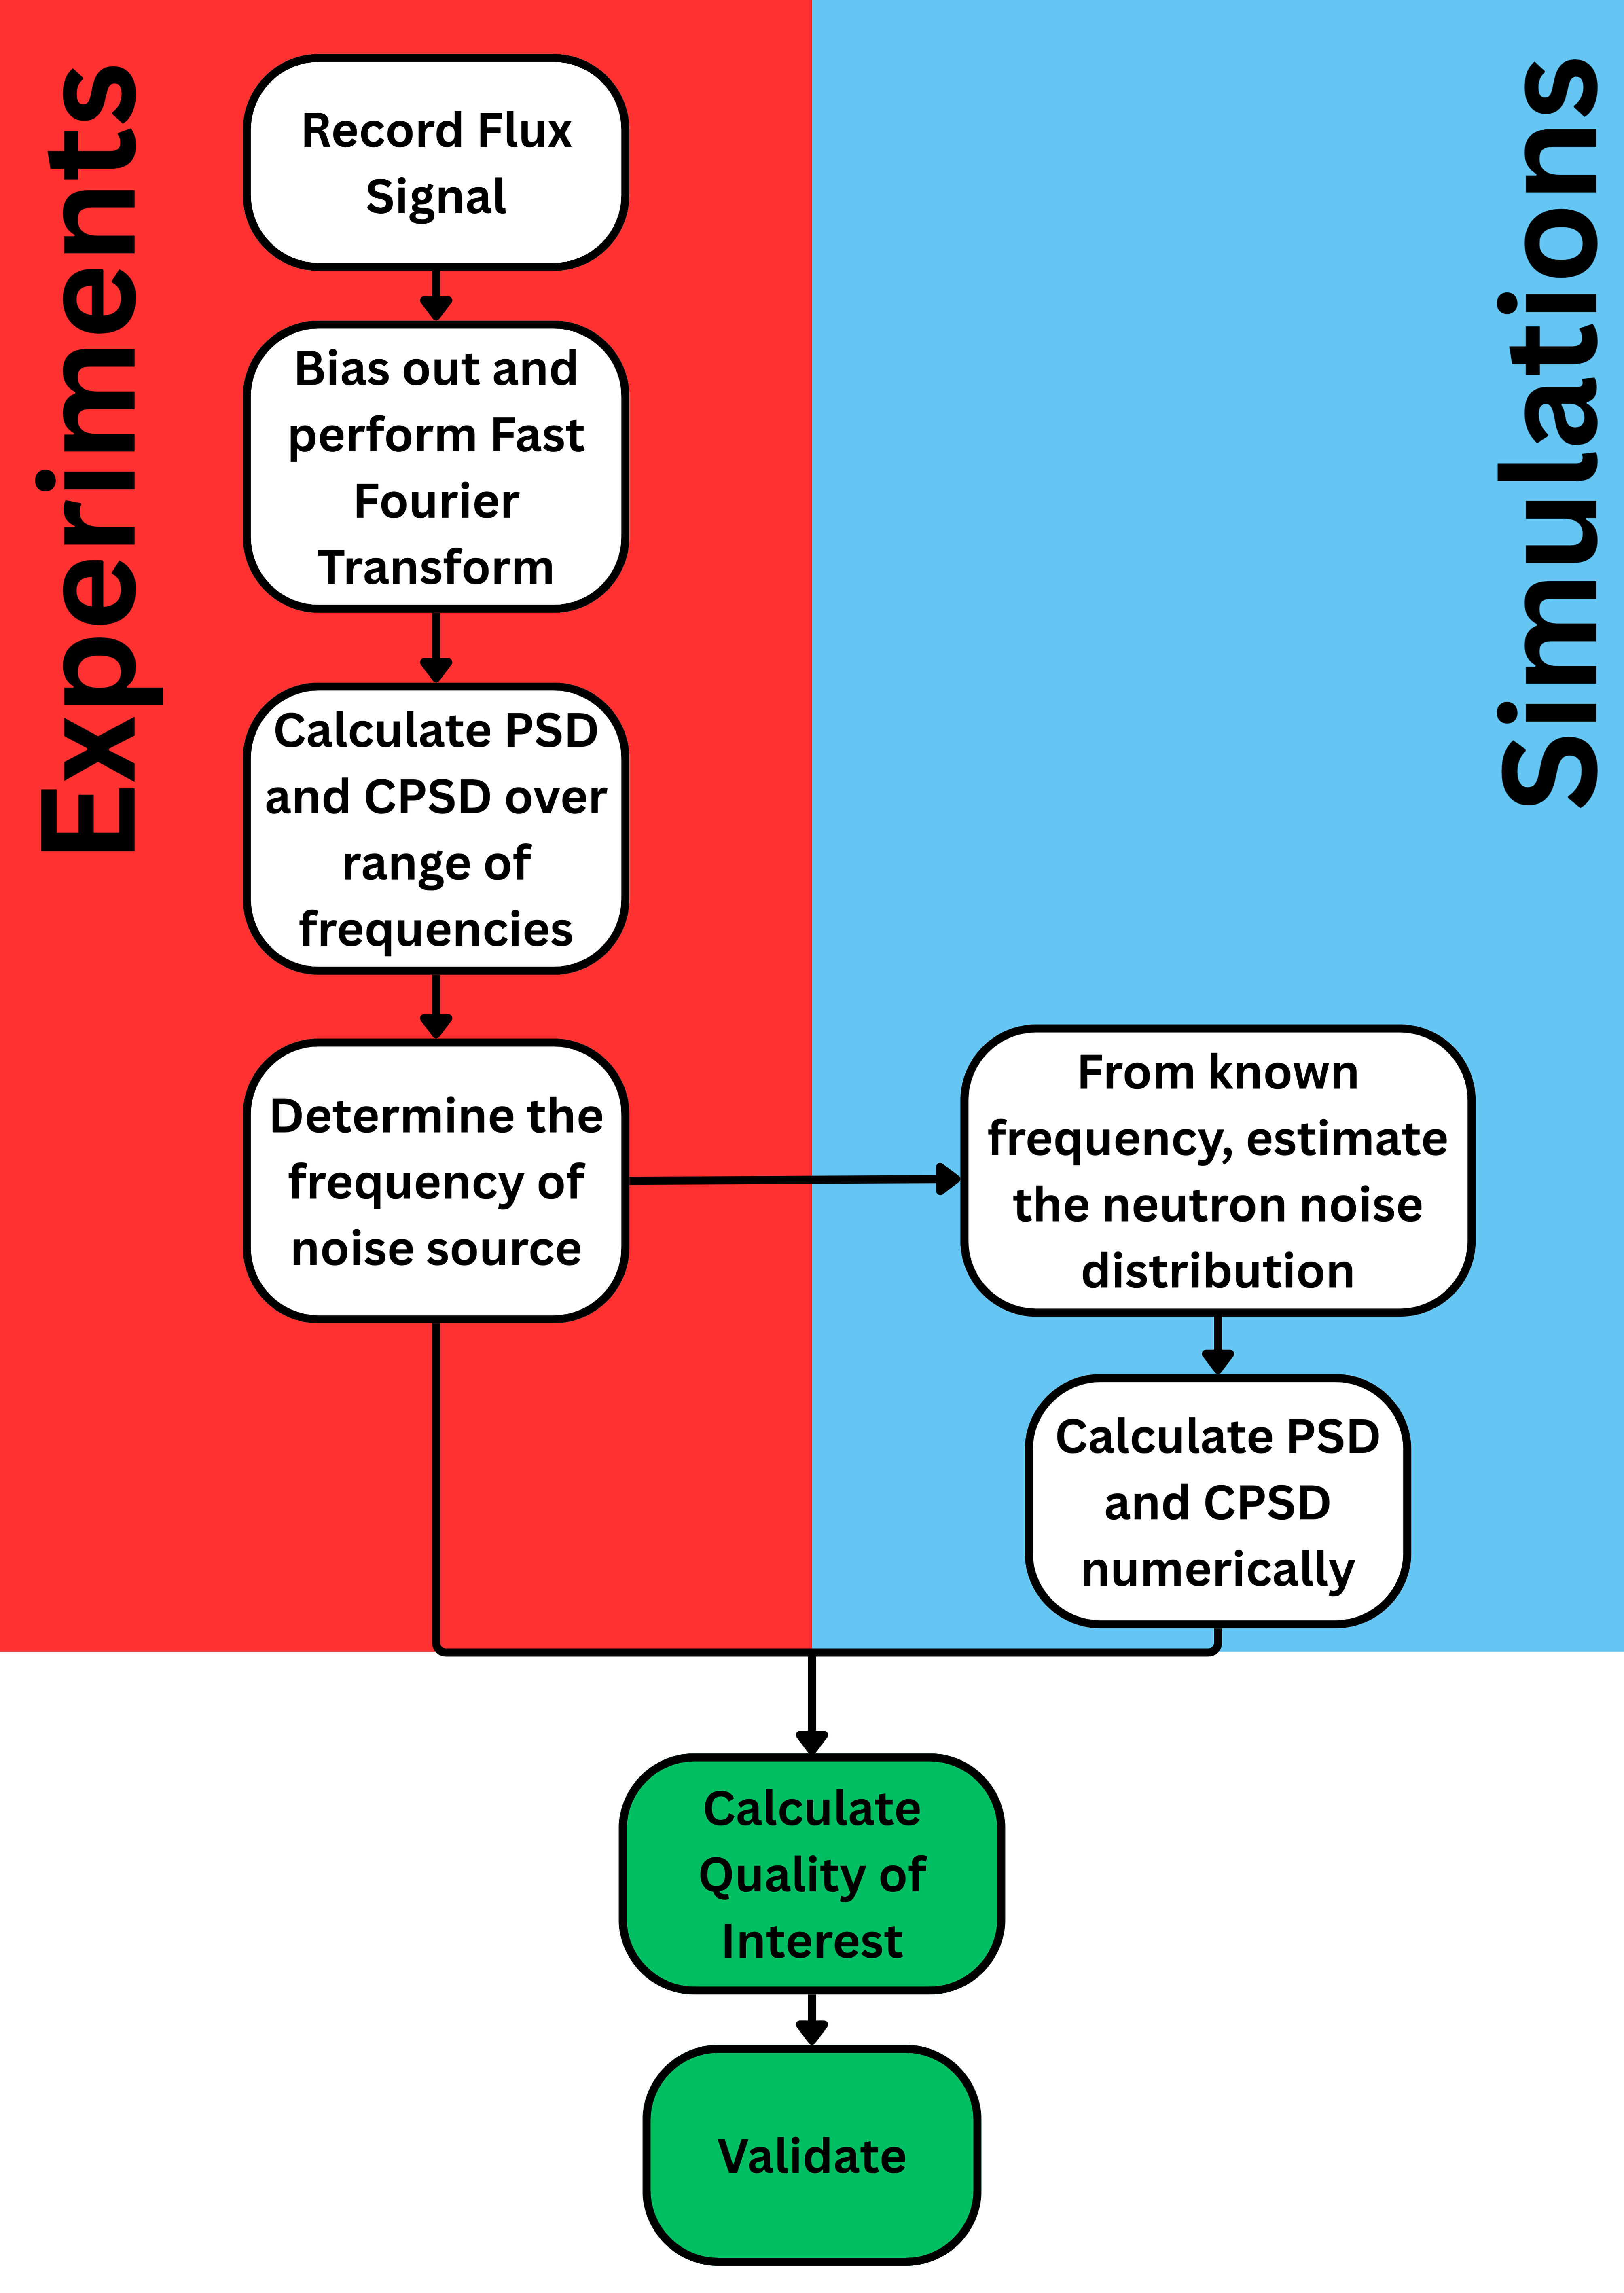
\includegraphics[width=0.5\textwidth]{figures/noise_workflow_exp1.png}
        \caption{General workflow of neutron noise experiment and simulation}
        \label{fig:flow_diagram}
\end{figure}

Assuming $\delta \phi_g (\textbf{r},\omega)$ is known from the computational method, the PSD can be determined using Welch method as follow \cite{mylonakisCORESIMSimulations2021}:

\begin{equation}
        \text{CPSD}_{xy} = \biggl(\frac{\delta \phi_{g}(\textbf{r}, \omega)}{\phi_{g}(\textbf{r})} \biggr)_x^* \cdot \biggl(\frac{\delta \phi_{g}(\textbf{r}, \omega)}{\phi_{g}(\textbf{r})} \biggr)_y
        \label{eq:CPSD_comp}
\end{equation}

To further understand the physical meaning of neutron noise, we can utilize point kinetic approximations to extract the integral parameters that characterize the reactor. To do this, we start by factorizing the time-dependent forward flux into its amplitude and shape function, such that,
\begin{equation}
        \phi (\textbf{r}, E, t) = P(t) \psi (\textbf{r}, E, t)
\end{equation}
with the following normalization condition,
\begin{equation}\label{eq:normalization}
        \frac{\partial}{\partial t} \int_{\textbf{E}} \int_{\textbf{r}} \biggl( \frac{1}{v} \phi^{\dagger}(\textbf{r}, E) \psi (\textbf{r}, E, t) \biggr) d\textbf{r} dE = 0
\end{equation}
In this case, $\phi^{\dagger}(\textbf{r}, E)$ is the solution of the adjoint equation. The normalization in Eq. \ref{eq:normalization} comes from the constraint of the variation of the flux shape in point-kinetic approximations. By having this constraint, the time dependence of the flux will largely be carried away by the amplitude function \cite{ottIntroductoryNuclearReactor1985}. Then, we split all the time-dependent components into the main values and the perturbations. Here, we define the initial condition (mean value) of the forward flux as follows,
\begin{equation}
        \phi_0(\textbf{r}, E) = P_0 \psi_0 (\textbf{r}, E)
\end{equation}
Therefore, we can write the neutron noise as follows (neglecting second-order terms),
\begin{equation}
        \begin{aligned}
                \delta \phi(\textbf{r}, E, t) &= \phi (\textbf{r}, E, t) - \phi_0(\textbf{r}, E)\\
                &= (P(t)\psi(\textbf{r}, E, t)) - \phi_0(\textbf{r}, E)\\
                &= \biggl( P_0 + \delta P(t) \biggr) \biggl( \psi_0(\textbf{r}, E)+\delta \psi(\textbf{r}, E, t) \biggr) - \phi_0(\textbf{r}, E) \\
                &= \biggl( P_0 \psi_0(\textbf{r}, E) \biggr) + \biggl(  \delta P(t) \psi_0(\textbf{r}, E)\biggr)+ \biggl(P_0 \delta \psi(\textbf{r}, E, t) \biggr) + \biggl( \delta P(t) + \delta \psi(\textbf{r}, E, t) \biggr) - \phi_0(\textbf{r}, E) \\
                &= \biggl(  \delta P(t) \psi_0(\textbf{r}, E)\biggr)+ \biggl(P_0 \delta \psi(\textbf{r}, E, t) \biggr)\\
                &= \delta P(t) \frac{\phi_0(\textbf{r}, E)}{P_0} + P_0 \delta \psi(\textbf{r}, E, t)
        \end{aligned}
        \label{eq:noise_component_time}
\end{equation}
Applying Fourier transforms to Eq. \ref{eq:noise_component_time} yields the following.
\begin{equation}\label{eq:noise_component_freq}
        \delta \phi(\textbf{r}, E, \omega) = \phi_0(\textbf{r}, E) \frac{ \delta P(\omega)}{P_0} + P_0 \delta \psi(\textbf{r}, E, \omega)
\end{equation}

Eq. \ref{eq:noise_component_freq} shows that the neutron noise can be split into two components. The first term on the right-hand side is the point-kinetic component, and the second is the spatial component of neutron noise. The point-kinetic component is driven by the reactivity effect of the perturbation, and the spatial component is driven by the nonuniform (in space) character of the perturbation \cite{pazsitNoiseTechniquesNuclear2010}.

The magnitude of power perturbation $\frac{\delta P(\omega)}{P_0}$ can be determined as follows. We can multiply Eq \ref{eq:noise_component_freq} by $\phi^{\dagger}(\textbf{r})/v$ and integrate over all the spatial and energy domains, which leads to the following.
\begin{equation}
        \int_{\textbf{E}} \int_{\textbf{r}} \frac{1}{v} \phi^{\dagger}(\textbf{r}, E) \delta \phi(\textbf{r}, E, \omega) d\textbf{r} dE = \frac{ \delta P(\omega)}{P_0} \int_{\textbf{E}} \int_{\textbf{r}} \frac{1}{v} \phi^{\dagger}(\textbf{r}, E) \phi_0(\textbf{r}, E) d\textbf{r} dE + P_0 \int_{\textbf{E}} \int_{\textbf{r}} \frac{1}{v} \phi^{\dagger}(\textbf{r}, E) \delta \psi(\textbf{r}, E, \omega) d\textbf{r} dE
        \label{eq:pk_long}
\end{equation}

Recall from Eq. \ref{eq:normalization}, we can split the shape function as follows:
\begin{equation}\label{eq:normalization_split}
\begin{aligned}
        \frac{\partial}{\partial t} \int_{\textbf{E}} \int_{\textbf{r}} \biggl( \frac{1}{v} \phi^{\dagger}(\textbf{r}, E) (\psi_0 (\textbf{r}, E) + \delta \psi (\textbf{r}, E, t) \biggr) d\textbf{r} dE &= 0 \\
        \frac{\partial}{\partial t} \int_{\textbf{E}} \int_{\textbf{r}} \biggl( \frac{1}{v} \phi^{\dagger}(\textbf{r}, E) \psi_0 (\textbf{r}, E) \biggr) d\textbf{r} dE + \frac{\partial}{\partial t} \int_{\textbf{E}} \int_{\textbf{r}} \biggl( \frac{1}{v} \phi^{\dagger}(\textbf{r}, E) \delta \psi (\textbf{r}, E, t) \biggr) d\textbf{r} dE &= 0 \\
        \frac{\partial}{\partial t} \int_{\textbf{E}} \int_{\textbf{r}} \biggl( \frac{1}{v} \phi^{\dagger}(\textbf{r}, E) \delta \psi (\textbf{r}, E, t) \biggr) d\textbf{r} dE &= 0 \\
\end{aligned}
\end{equation}

This means that Eq. \ref{eq:pk_long} can be simplified as follows:
\begin{equation}
        \frac{ \delta P(\omega)}{P_0} = \frac{\int_{\textbf{E}} \int_{\textbf{r}} \frac{1}{v} \phi^{\dagger}(\textbf{r}) \delta \phi(\textbf{r}, \omega) d\textbf{r} dE}{\int_{\textbf{E}} \int_{\textbf{r}} \frac{1}{v} \phi^{\dagger}(\textbf{r}) \phi_0(\textbf{r}) d\textbf{r} dE}
\end{equation}

Continuing with the derivation of the point kinetics component, we start from the time-dependent neutron diffusion equation, multiply both sides with adjoint flux as a weighting function, and integrate over the spatial domain, yielding the following:
\begin{equation}
    \begin{aligned}
        \frac{dP_0}{dt} + \frac{d(\delta P(t))}{dt} &= \frac{\rho_0}{\Lambda} (P_0 + \delta P(t)) + \frac{\delta \rho(t)}{\Lambda} (P_0 + \delta P(t)) - \frac{\beta}{\Lambda} (P_0 + \delta P(t)) + \lambda (C_0 + \delta C(t))\\
        \frac{dC_0}{dt} + \frac{d(\delta C(t))}{dt} &= \frac{\beta}{\Lambda} (P_0 + \delta P(t)) - \lambda (C_0 + \delta C(t))\\
    \end{aligned}
\end{equation}

By neglecting second-order terms and eliminating the time-independent component, we can simplify the equation into:
\begin{equation}
    \begin{aligned}\label{eq:simple_PRKE}
        \frac{d(\delta P(t))}{dt} &= \frac{\delta \rho(t)}{\Lambda} P_0 - \frac{\beta}{\Lambda} \delta P(t) + \lambda \delta C(t)\\
        \frac{d(\delta C(t))}{dt} &= \frac{\beta}{\Lambda} \delta P(t) - \lambda \delta C(t)\\
    \end{aligned}
\end{equation}
Applying the Fourier Transform to Eq. \ref{eq:simple_PRKE} yields to:
\begin{equation}
    \begin{aligned}\label{eq:simple_PRKE_omega}
        i \omega \delta P(\omega) &= \frac{P_0}{\Lambda} \delta \rho(\omega) - \frac{\beta}{\Lambda} \delta P(\omega) + \lambda \delta C(\omega)\\
        i \omega \delta C(\omega) &= \frac{\beta}{\Lambda} \delta P(\omega) - \lambda \delta C(\omega)\\
    \end{aligned}
\end{equation}
where $\omega = 2 \pi f$. Simplifying the precursor equation of Eq. \ref{eq:simple_PRKE_omega}, yields:
\begin{equation}
    \begin{aligned}\label{eq:simple_PRKE_precursor}
        \delta C(\omega) &= \frac{\beta}{\Lambda (i \omega + \lambda)} \delta P(\omega)\\
    \end{aligned}
\end{equation}
Then, substituting Eq. \ref{eq:simple_PRKE_precursor} to the power equation of Eq. \ref{eq:simple_PRKE_omega}, yields to:
\begin{equation}
    \begin{aligned}\label{eq:simple_power_omega}
        i \omega \delta P(\omega) &= \frac{P_0}{\Lambda} \delta \rho(\omega) - \frac{\beta}{\Lambda} \delta P(\omega) + \frac{\lambda \beta}{\Lambda (i \omega + \lambda)} \delta P(\omega)\\
        \frac{P_0}{\Lambda} \delta \rho(\omega) &= \biggl( i \omega +  \frac{\beta}{\Lambda} - \frac{\lambda \beta}{\Lambda (i \omega + \lambda)} \biggr) \delta P(\omega) \\
        \delta P(\omega) &= \delta \rho(\omega)P_0 \frac{1}{\Lambda \biggl( i \omega +  \frac{\beta}{\Lambda} - \frac{\lambda \beta}{\Lambda (i \omega + \lambda)} \biggr)} \\
        \delta P(\omega) &= \delta \rho(\omega)P_0 G(\omega)\\
    \end{aligned}
\end{equation}
Since we derive Eq. \ref{eq:simple_power_omega} from Eq. \ref{eq:freq_4}, we can explicitly define $\delta \rho(\omega)$ as follows,
\begin{equation}
        \delta \rho(\omega) = \frac{\int_{\textbf{E}} \int_{\textbf{r}} \phi^{\dagger}(\textbf{r}, E) \textbf{S}(\textbf{r}, E, \omega) d\textbf{r} dE}{\int_{\textbf{E}} \int_{\textbf{r}} \phi^{\dagger}(\textbf{r}, E) \textbf{F}(\textbf{r}, E) d\textbf{r} dE}
\end{equation}
where $\textbf{S}(\textbf{r}, \omega)$ is the noise source in the system, and $\textbf{F}(\textbf{r})$  is the fission source in the forward equation. This means that we have two ways to calculate the zero-power reactor transfer function $G(\omega)$. They are,
\begin{equation}\label{eq:ZPRTF}
        G(\omega) = \frac{1}{\Lambda \biggl( i \omega +  \frac{\beta}{\Lambda} - \frac{\lambda \beta}{\Lambda (i \omega + \lambda)} \biggr)} = \frac{\delta P (\omega) /P_0}{\delta \rho(\omega)}
\end{equation}

The zero-power reactor transfer function is one method for observing system’s behavior during a small sinusoidal perturbation. It could also be used to check whether the reactivity feedback is as expected from the design \cite{bellNuclearReactorTheory1970}. The input in ZPRTF is the reactivity perturbations ($\delta \rho (\omega)$), and the output is the power perturbations ($\frac{\delta P(\omega)}{P_0}$). It should be noted that even though the transfer function is called the zero-power reactor transfer function, Eq. \ref{eq:ZPRTF} only captures the $\delta \rho (\omega)$ response driven by the point kinetic component of the neutron noise. Therefore, it is more appropriate to call the zero-power reactor transfer function as the point kinetic zero-power reactor transfer function. An example of ZPRTF is given in Figure \ref{fig:Example2DTransferFunction}.

We can see from Figure \ref{fig:Example2DTransferFunction}, at lower frequencies, the magnitude of ZPRTF increases as the frequency decreases. This increases the point kinetic component of neutron noise, which makes the magnitude of neutron noise increases. This means that the neutron noise is dominated by the point kinetic component. At higher frequencies, the opposite happens. The magnitude of ZPRTF decreases as the frequency increases, which decreases the point kinetic component of neutron noise. In this case, the contribution of the point kinetic component to the neutron noise decreases. This means that the contribution of spatial component becomes more significant. At mid-frequencies, it is observed that there will be a plateau region in the magnitude of the transfer function in the range of $[\lambda ; \beta/\Lambda_0]$. In this region, the amplitude is nearly constant and equal to $1/\beta$. The phase of the transfer function generally will be similar to a bell curve, where the peak of the curve of the phase is close to zero \cite{demaziereDevelopmentPointkineticVerification2017}.

\begin{figure}[H]
        \centering
        \begin{subfigure}{.48\textwidth}
          \centering
          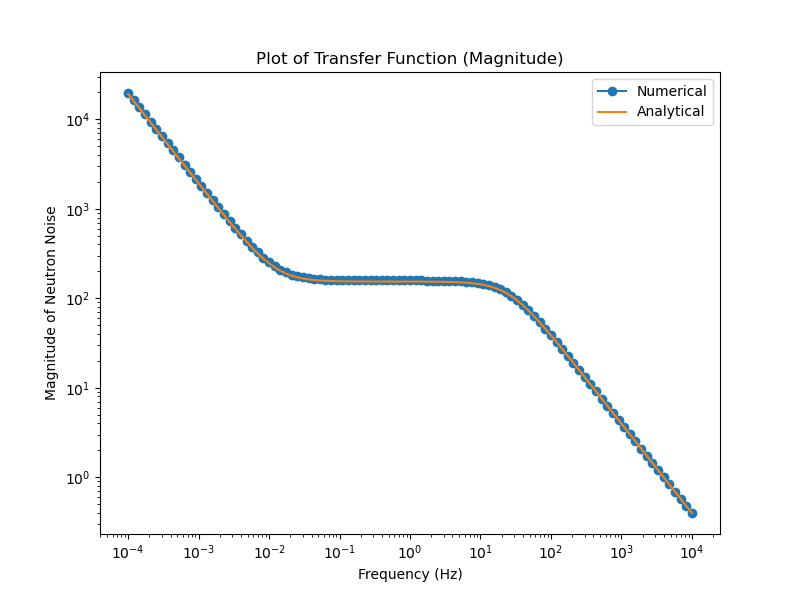
\includegraphics[width=\linewidth]{figures/OBJECTIVES3_TEST01_2DMG_BIBLIS_AVS_NOISE_Magnitude_freq.png}
        \end{subfigure}
        \hfill
        \begin{subfigure}{.48\textwidth}
          \centering
          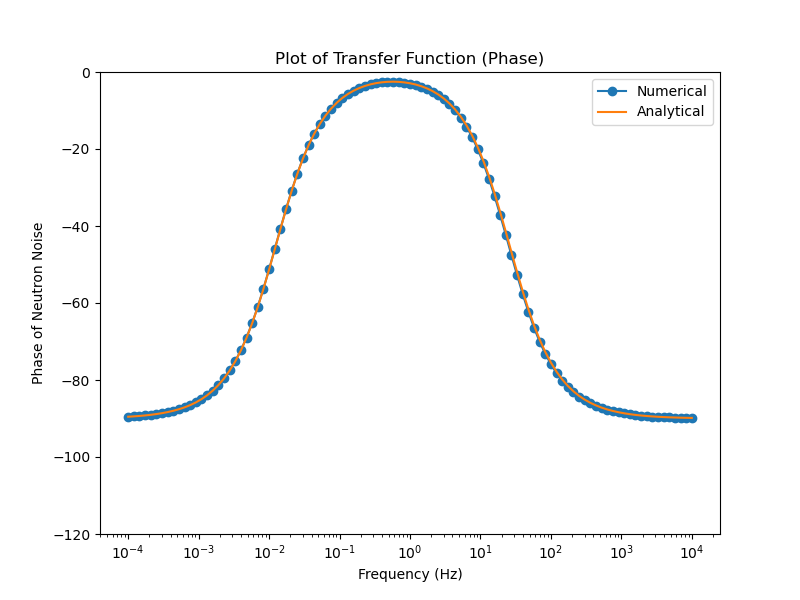
\includegraphics[width=\linewidth]{figures/OBJECTIVES3_TEST01_2DMG_BIBLIS_AVS_NOISE_Phase_freq.png}
        \end{subfigure}
        \caption{Magnitude (left) and phase delay (right) of transfer function in 2D BIBLIS Benchmark}
        \label{fig:Example2DTransferFunction}
\end{figure}

\subsection{Neutron Noise Models and Sources}

In the computational method, neutron noise sources can generally be divided into two categories. The first category is the absorber of variable strength, and the second category is called the vibrating absorber. 

\subsubsection{Absorber of Variable Strength}

Although terminology specifies absorber, these types of noise typically refer to any type of cross-sections. This includes absorption, fission, and scattering  \cite{pazsitNoiseTechniquesNuclear2010}. The absorbers of variable strength can be represented as fluctuations in the macroscopic cross-section at a given fixed location $\textbf{r}_0$ and the noise sources can be expressed as:
\begin{equation}\label{eq:AVS_FGW}
        \delta \Sigma_x (\textbf{r}, \omega) = \gamma (\omega) \delta (\textbf{r} - \textbf{r}_0)
\end{equation}
where $\gamma (\omega)$ is the noise source strength. Eq. \ref{eq:AVS_FGW} is also called the Feinberg-Galanin-Williams model \cite{pazsitNoiseTechniquesNuclear2010}. Some examples of this type of noise include the perturbations traveling with the coolant flow \cite{jonssonTwogroupTheoryNeutron2011} and perturbations due to unseated fuel assembly \cite{demaziereAnalysisMethodsDetermination2006}. In terms of modeling the noise source in a numerical tool, the absorber of variable strength can be intuitively modeled as a perturbation of cross-section in the center of computational node \cite{mylonakisCORESIMFlexible2021}. 

\subsubsection{Vibrating Absorber}

The second category is the vibrating absorber. The vibrating absorber could include vibration of the fuel assembly \cite{chionisSIMULATE3KAnalysesNeutron2017}, vibration of control rods \cite{pazsitNeutronNoiseDiagnostics1983}, or vibration of the core barrel \cite{pazsitDevelopmentsCoreBarrelMotion2016}. In the vibration absorber, the perturbation is modeled as the displacement of the vibrating assembly (or another component) from its nominal position. This is done by assuming that the neutron noise is induced by vibrating interfaces.

We can use one-dimensional perturbation as an example. Let’s assume that we have a one-dimensional system that is vibrating in one interface. We denote the equilibrium position of the vibrating interface as $x_0$. Then, we define $\Sigma_\alpha^L$ and $\Sigma_\alpha^R$ as macroscopic cross sections of the region at the left ($x<x_0$) and at the right ($x>x_0$) of the vibrating interface. We assume that the vibration in the interface is periodic with frequency $\omega_0$, and amplitude $\varepsilon$, which is smaller than the side $d$ of the region of interest in the interface perturbation. Figure \ref{fig:1Dvibration} illustrates the vibrating absorber case in 1D \cite{zoiaAnalysisNeutronNoise2021}.
\begin{figure}[H]
        \centering
        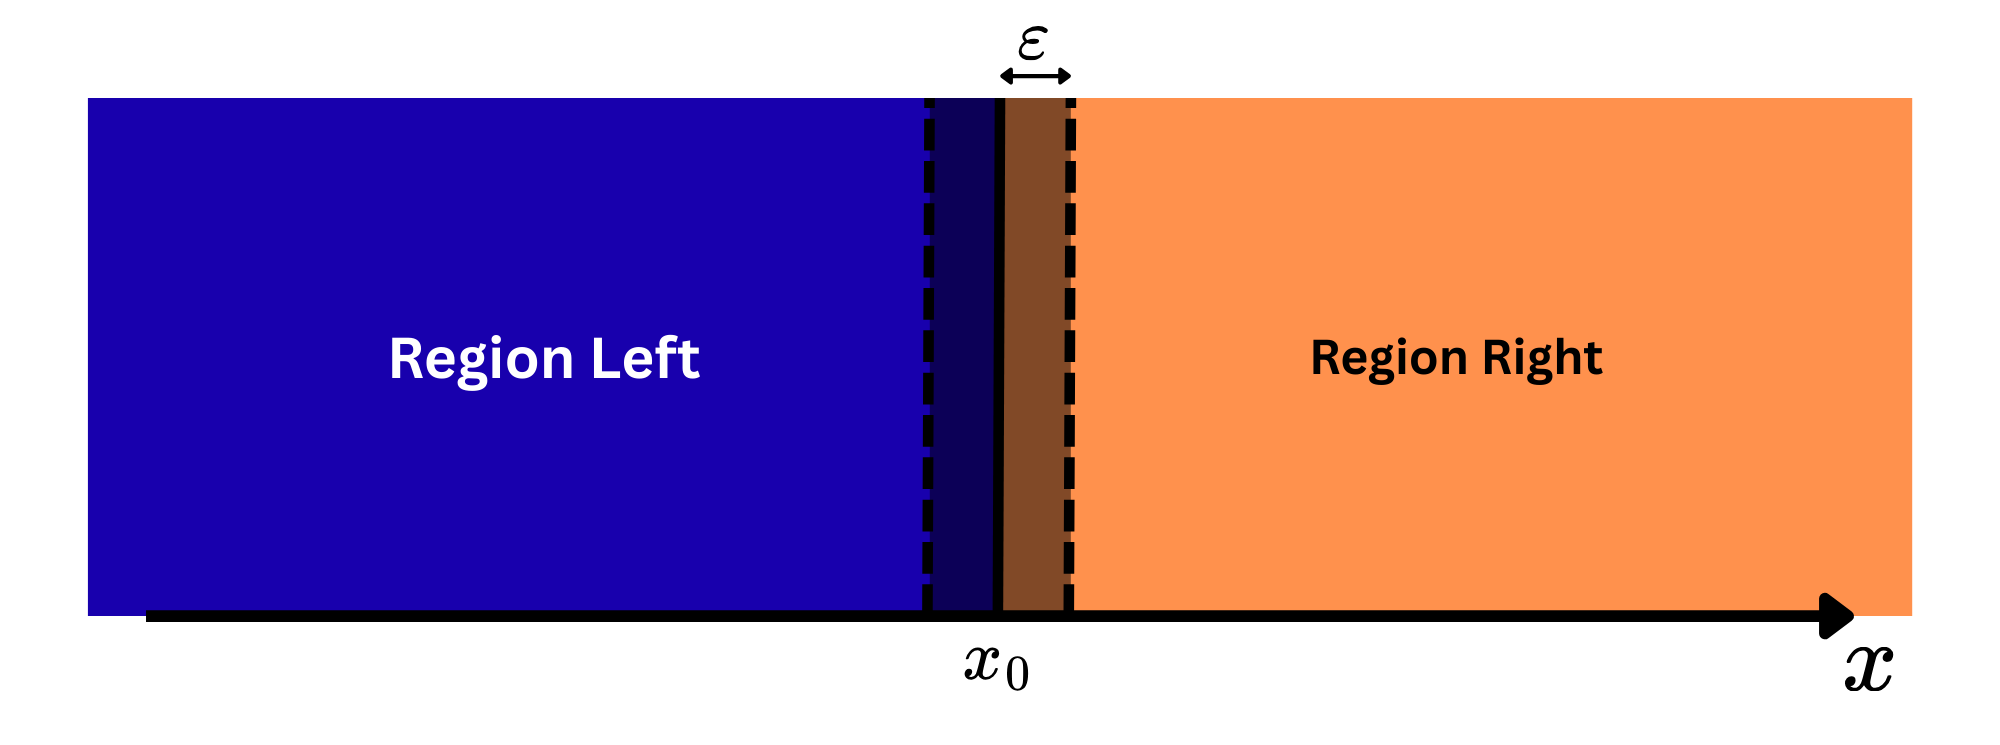
\includegraphics[width=0.5\textwidth]{figures/Region Left.png}
        \caption{Example of vibrating absorber noise source in 1D}
        \label{fig:1Dvibration}
\end{figure}

In this case, the position of the moving interface $x_i (t)$ and the perturbation $\delta\Sigma_\alpha (x, E, t)$ can be written as follows:
\begin{equation}
    x_i(t) = x_0 + \varepsilon \sin(\omega_0 t)
\end{equation}
\begin{equation}\label{eq:dABS_exact}
    \delta\Sigma_\alpha (x, E, t) = \biggl(\Sigma_\alpha^L (x, E)-\Sigma_\alpha^R (x, E)\biggr) \biggl( H(x-x_0)-H(x-x_0-\varepsilon \sin(\omega_0 t) \biggr)
\end{equation}

Where $H(x-x_0)$ is the Heaviside function. This means that the value of $\delta\Sigma_\alpha (x, E, t)$ is non-zero only at the perturbed area, which $x-\varepsilon \leq x \leq x+\varepsilon$ \cite{zoiaAnalysisNeutronNoise2021}. From Eq. \ref{eq:dABS_exact}, we can perform Fourier transformations by dividing into two different regions, $x<x_0$ and $x>x_0$. This will lead to the definition of the neutron noise source for periodic vibrating absorber. 

For $\varepsilon\ll d$, one could perform an approximation called the weak absorber approximation, also known as the $\varepsilon/d$ model \cite{pazsitInvestigationSpaceDependentNoise1977}. This model indicates that the magnitude of the perturbation is so small compared to the reactor size that it can be converted into a spatially localized cross-section perturbation. The weak absorber approximation is done by performing a Taylor series expansion to Eq. \ref{eq:dABS_exact} in powers of $\varepsilon$, which yields the following:
\begin{equation}\label{eq:dABS_taylor}
    \delta\Sigma_\alpha (x, E, t) = \biggl(\Sigma_\alpha^L (x, E)-\Sigma_\alpha^R (x, E)\biggr) \biggl( \varepsilon \sin(\omega_0 t) \delta(x-x_0)-\frac{\varepsilon^2 \sin^2(\omega_0 t)}{2} \delta'(x-x_0)+ ... \biggr)
\end{equation}
Performing Fourier transform to Eq. \ref{eq:dABS_taylor} yields the following:
\begin{equation}\label{eq:dABS_taylor_omega}
    \delta\Sigma_\alpha (x, E, \omega) = \biggl(\Sigma_\alpha^L (x, E)-\Sigma_\alpha^R (x, E)\biggr) \biggl( -i \pi \varepsilon \delta(x-x_0) \delta(\omega-\omega_0)-\frac{\pi}{4} \varepsilon^2 \delta'(x-x_0) \delta(\omega-2\omega_0)+ ... \biggr)
\end{equation}

From Eq. \ref{eq:dABS_taylor_omega}, we can see that the periodic vibration can be approximated as a series of frequencies \cite{zoiaAnalysisNeutronNoise2021}. Some literature shows that the second harmonic might be relevant in some cases \cite{luciaCorrelationNeutronNoise1973, pazsitInvestigationSpaceDependentNoise1977, pazsitLinearizationVibrationinducedNoise1984}. However, previous works in $\varepsilon/d$ approximation only consider the first order effect, which yields the following.
\begin{equation}\label{eq:dABS_taylor_omega_truncated}
    \delta\Sigma_\alpha (x, E, \omega) = \biggl(\Sigma_\alpha^L (x, E)-\Sigma_\alpha^R (x, E)\biggr) \biggl( -i \pi \varepsilon \delta(x-x_0) \delta(\omega-\omega_0) \biggr)
\end{equation}
In terms of modeling the noise source in a numerical tool, the vibrating absorbers can be modeled as a perturbation of cross-sections at the boundary of the vibrating region \cite{mylonakisCORESIMFlexible2021}.

The vibrating absorber model shown in this chapter (which will be used for the remainder of the dissertation) comes from the linearization of vibration-induced noise, which yields an idealized delta function that eventually leads to Eq. \ref{eq:dABS_taylor_omega_truncated}.  When this absorber model is applied as the noise source in Eq. \ref{eq:freq_4}, it will provide accurate estimates for the neutron noise when $\varepsilon/d \ll 1$. Linearization of the vibrating absorber model means that the system only responds at frequency $\omega_0$. This brings up the issue of an effect called the “double frequency” effect, which means that a system subject to a periodic vibration at frequency $\omega_0$ could have a secondary peak at frequency $2\omega_0$. This double-frequency effect has been demonstrated in some experiments \cite{luciaCorrelationNeutronNoise1973}. By linearizing the vibration noise source, the secondary peak is no longer observable.  

\section{Existing Computational Tools of Neutron Noise Analysis}
\label{sec:noise_tools}

\subsection{Solving Neutron Noise Problems using Deterministic Methods}

Deterministic transport methods have been developed to solve the neutron noise equation. It should be noted that knowledge of the forward neutron flux distribution and k-criticality is necessary to perform neutron noise simulations, as these parameters become the input to the neutron noise simulation. The tools developed varied in terms of spatial discretization, energy discretization, angular discretization, and the domain of interest to solve the neutron noise equation. The following list shows the development of neutron noise simulation tools using deterministic methods. This list is sorted based on the time at which the literature has been published.
\begin{itemize}
    \item Demazi\`ere developed a 2-group, 2-dimensional (cartesian) neutron noise simulator in frequency domain. The simulator used finite difference for spatial discretization. The simulator calculated the neutron noise and the corresponding adjoint functions \cite{demaziereDevelopment2D2group2004}.
    \item Malmir et al. developed a 2-group, 2-dimensional neutron noise simulator for hexagonal geometries. The neutron noise simulator is in frequency domain. The box-scheme finite difference method for hexagonal mesh was used for spatial discretization. The spatial discretization is performed by splitting each hexagon into seven hexagonal mesh boxes. The simulation of neutron noise in VVER-1000 has been applied to this simulator \cite{malmirDevelopment2D2group2010}.
    \item Larsson et al. developed a 2-group, 2-dimensional (cartesian) neutron noise simulator in frequency domain. The simulator used analytical nodal method (ANM) for spatial discretization. ANM is used to solve for both forward flux and neutron noise calculations \cite{larssonNeutronNoiseCalculations2011}.
    \item Demazi\`ere developed a multi-purpose neutronic tool called CORE SIM. CORE SIM is a 2-group, 3-dimensional (cartesian) simulator. It uses finite difference for spatial discretization. It has the capability to solve forward, adjoint, and neutron noise equations. The neutron noise equation is solved in frequency domain \cite{demaziereCORESIMMultipurpose2011}.
    \item Tran et al. developed a tool for neutron noise equation in hexagonal geometries. The tool is a multigroup, 2-dimensional (hexagonal) simulator. It uses finite difference for spatial discretization. It has been compared with analytical solutions based on 2-dimensional 2-group homogeneous systems \cite{tranNeutronNoiseCalculations2013}.
    \item Rouchon et al. developed a neutron noise tool in the APOLLO3. APOLLO3 is a 3-dimensional (cartesian) multigroup diffusion tool. It uses Nodal Expansion Method (NEM) for spatial discretization \cite{schneiderAPOLLO3CEADeterministic2016}. The neutron noise simulation is performed using frequency domain. In APOLLO3, the neutron noise simulation is performed by changing the production operator into complex number, and adding an iteration loop between the real and imaginary parts of the neutron noise equation \cite{rouchonNew3DMultigroup2017}.
    \item Rohde et al. simulated neutron noise in time domain using DYN3D. DYN3D is a three-dimensional best-estimate tool for simulating steady states and transients of LWRs \cite{rohdeReactorDynamicsCode2016}. The neutron noise simulation is performed for a generic KONVOI reactor core. The neutron noise is induced by coolant inlet temperature variations, channel-wise mass-flow rate variation, and variation in the local moderator density in a part of the core \cite{rohdeNeutronNoiseObservations2018}.
    \item Chionis et al. developed a neutron noise tool in the SIMULATE-3K code (S3K). S3K is 2-group nodal code for transient analysis. For neutron noise simulation, the code uses time domain analysis. The code is applied to analyze fuel assembly vibration in the Swiss PWR \cite{chionisSIMULATE3KAnalysesNeutron2017}. The same tool is also used to simulate fuel assembly vibrations in KWU pre-KONVOI reactors \cite{vermaModellingAnalysisFuel2021}.
    \item Bahrami et al. developed a neutron noise tool based on SN method. The neutron noise equation is solved using Green’s function in frequency domain. The tool has been applied to several benchmarks problems and compared to diffusion-based neutron noise tool. The results show that the difference between SN-based and diffusion-based methods are noticeable in the media with less than 100 mean free path thickness as well as source locations near the edge. In these cases, more comprehensive tests are necessary \cite{bahramiSNTransportMethod2018}.
    \item Vidal-Ferrandiz et al. developed FEMFFUSION. FEMFFUSSION is a 3-dimensional, 2-group neutron diffusion simulator that uses a finite element method to solve the neutron diffusion equation. FEMFFUSION solves the neutron noise equation in the time domain \cite{vidal-ferrandizNeutronicSimulationFuel2020}.
    \item Mylonakis et al. developed CORE SIM+, which is the extension of CORE SIM. CORE SIM+ has the capability to solve non-unform meshes. It also has the capability to generate Green’s functions for solving neutron noise equation \cite{mylonakisCORESIMFlexible2021}.
    \item Gong et al. developed a prototype code called CORCA-NOISE. CORCA-NOISE is a multigroup neutron noise tool based on the simplified P3 method for the angular discretization. It is part of the industry SP3 tool CORCA-PIN, which is developed by the Nuclear Power Institute of China (NPIC). It uses finite element method for spatial discretization. This tool has been compared to CORE SIM for two benchmark studies \cite{gongNeutronNoiseCalculation2021}.
    \item Yi et al. developed a neutron noise tool called the NOISE-SN. NOISE-SN is a multigroup, 3-dimensional (cartesian) neutron noise tool based on the SN method for angular discretization. It uses diamond finite difference for the spatial discretization. The tool is compared with CORE SIM+ using C4V and C5G7 benchmarks \cite{yiSimulationNeutronNoise2021}.
\end{itemize}

\subsection{Solving Neutron Noise Problems using Monte Carlo Methods}

Monte Carlo method has been used to solve neutron noise equations. Several methods are developed to solve the neutron noise equation from transport theory. Some others developed Monte Carlo method to solve Green’s function using Monte Carlo. Compared to a conventional fixed source transport equation, the neutron noise equation (see Eq. \ref{eq:freq_4}) has three main differences. First, the solution of neutron noise equation, $\delta \phi(\textbf{r},\Omega, E, \omega)$, is a complex value. Second, the production term is multiplied by a complex-value factor $\biggl( \chi^p_g (1-\beta_{\text{eff}}) + \chi^d_g \frac{\lambda \beta_{\text{eff}}}{i \omega + \lambda} \biggr)$. Third, the addition of $\frac{i \omega}{v} \delta \phi(\textbf{r},\Omega, E, \omega)$ in the equation. The following list shows the use of Monte Carlo method to solve neutron noise equation.
\begin{itemize}
    \item Yamamoto developed a method to solve neutron noise equations using Monte Carlo method \cite{yamamotoMonteCarloMethod2013}. The method is developed based on the neutron leakage-corrected calculation using complex-weighted Monte Carlo method \cite{yamamotoMonteCarloMethod2012}. The strategy of solving neutron noise equation using Monte Carlo method is divided into three parts. First, the method introduces complex-valued weights for each simulated neutron noise particle. These weights can have positive or negative signs. Second, as the particle transported, the method performed weight cancellation of positive and negative weights. The weight cancellation is necessary to avoid the production of too many neutron noise particles at low and very high frequencies. Third, the method includes the additional term $\frac{i \omega}{v} \delta \phi(\textbf{r},\Omega, E, \omega)$ during the random walk processes of the particles with complex-valued weights. For verification purposes, this method has been verified with analytical solutions and comparison with diffusion theory. The results show that the diffusion theory yields less accurate results compared to Monte Carlo method for higher frequency noise sources \cite{yamamotoMonteCarloMethod2013}.
    \item Rouchon et al. developed a new Monte Carlo-based method to solve neutron noise equation \cite{rouchonNewMonteCarlo2017}. Similar to \cite{yamamotoMonteCarloMethod2013}, the method is based on transporting complex-valued neutron noise particles. However, the method introduces a new term to the neutron noise equation $\frac{(\eta - i)}{\eta} \eta \frac{\omega}{v} \delta \phi (\textbf{r}, \omega)$, where $\eta$ is a real constant with the same sign as $\omega$. By having this modification, the method can use conventional algorithms for fixed source problems for all frequencies. This method also does not need any weight cancellation techniques for low and very high frequencies. This method has been compared to \cite{yamamotoMonteCarloMethod2013} and shows that the method has better Figure of Merit (FoM) compared to \cite{yamamotoMonteCarloMethod2013}.
    \item Demaziere et al. developed a Monte Carlo-based method that leverages Green’s function for solving neutron noise equation. Starting from neutron noise equation in frequency domain, the authors split the equation in coupled balance equation, representing the real part and imaginary part of neutron noise. To solve these coupled equations using Monte Carlo code, the reaction rates in each equation need to be positive. Demaziere et al. rewrote the coupled equation such that the reaction rates are positive. Then, the solution of neutron noise can be obtained using Green’s functions that are generated using Monte Carlo simulations \cite{demaziereMonteCarlobasedDynamic29}.
\end{itemize}

\section{Conclusion}

This chapter provides a general overview of neutron noise. Neutron noise analysis has been implemented in nuclear reactors, especially for anomaly detections. Computational methods of neutron noise have been derived and reviewed in this chapter. This chapter also derived the point kinetics approximation of neutron noise equation to obtain several parameters (e.g. power perturbations, reactivity perturbations, and zero-power reactor transfer functions). This chapter reviews different models of neutron noise sources and its implementation to computational method. This chapter also provides several tools that have been developed to solve neutron noise equation, both using deterministic and Monte Carlo methods.

%=======================================================================